% =====================================================================
\lecture{2}{\en{MCMC} וסופרנובות: מדידת האנרגיה האפלה}{שעתיים: חלק א' (שעה, סוף מפגש 1) --- בייס ו-\en{MCMC} על קו ישר; חלק ב' (שעה, מפגש 2) --- \en{Pantheon+} והמחברת \en{MCMC\_Pantheon\_he}.}
% =====================================================================

\begin{goalbox}
\textbf{מטרות.} (1) לנסח הסקה בייסיאנית: נראות, מוקדמת, מאוחרת, מרג'ינליזציה. (2) להבין את \en{Metropolis--Hastings} ו-\en{emcee}, ולדעת מתי מותר להאמין לשרשרת. (3) להחיל את אותה מכונה על 1590 סופרנובות ולמדוד $\Omega_m$ ו-$w$.
\end{goalbox}

\subsection*{חלק א' --- הסקה בייסיאנית ו-\en{MCMC}}

\subsection{משפט בייס}
\begin{equation}
\underbrace{P(\boldsymbol\theta|D)}_{\text{מאוחרת}}=\frac{\overbrace{\mathcal L(D|\boldsymbol\theta)}^{\text{נראות}}\ \overbrace{\pi(\boldsymbol\theta)}^{\text{מוקדמת}}}{\underbrace{P(D)}_{\text{עדות}}},
\qquad
\mathcal L\propto e^{-\chi^2/2},\quad \chi^2=\mathbf r^{\!\top}\mathsf C^{-1}\mathbf r,\quad \mathbf r=\mathbf d-\mathbf m(\boldsymbol\theta).
\end{equation}
למה בייס בקוסמולוגיה? יש יקום אחד, ואי אפשר לחזור על הניסוי. שואלים "מה סביר לגבי $\boldsymbol\theta$ בהינתן הנתונים", ולא "מה היה קורה בחזרות".

\textbf{מרג'ינליזציה.} תוצאה לפרמטר אחד מתקבלת באינטגרציה על כל השאר: $P(\theta_1|D)=\int P(\boldsymbol\theta|D)\,d\theta_2\cdots d\theta_n$. \emph{לא} מקבעים פרמטרי מטרד: אם $\rho$ הקורלציה בין שני פרמטרים, קיבוע אחד מהם מקטין את השגיאה על השני בפקטור $\sqrt{1-\rho^2}$ --- הערכת-חסר של השגיאה.

\subsection{למה לדגום, ואיך}
ב-$n$ פרמטרים רשת של 100 נקודות לציר עולה $100^n$ חישובי נראות. במקום זה יוצרים \textbf{שרשרת} של נקודות שהצפיפות שלהן פרופורציונלית למאוחרת; אז כל אינטגרל הוא ממוצע על הדגימות, וכל היסטוגרמה היא התפלגות שולית.

\begin{keybox}
\textbf{\en{Metropolis--Hastings}.} מנקודה $\boldsymbol\theta$:
\begin{enumerate}
\item מציעים $\boldsymbol\theta'=\boldsymbol\theta+\boldsymbol\epsilon$ (הצעה סימטרית, למשל גאוסית).
\item מחשבים $\alpha=\min\!\big[1,\;P(\boldsymbol\theta'|D)/P(\boldsymbol\theta|D)\big]$.
\item מקבלים את $\boldsymbol\theta'$ בהסתברות $\alpha$; אחרת \emph{חוזרים על} $\boldsymbol\theta$ בשרשרת.
\end{enumerate}
רק \emph{יחס} מאוחרות נכנס, ולכן העדות $P(D)$ לא נחוצה. שיווי משקל מפורט מבטיח שהשרשרת מתכנסת למאוחרת.
\end{keybox}
\textbf{\en{emcee}} (\en{Goodman--Weare}): אנסמבל של "הולכים"; כל הולך מציע צעד לאורך הקו אל הולך אחר (\en{stretch move}). הדוגם אינווריאנטי תחת טרנספורמציות אפיניות, ולכן מסתדר עם מאוחרות צרות ומשופעות בלי כיוונון גודל צעד.

\textbf{אבחון --- לפני שמדווחים מספר:}
\begin{itemize}
\item \textbf{\en{burn-in}:} השלכת החלק הראשון ($\sim5\tau$), שתלוי בנקודת ההתחלה.
\item \textbf{זמן אוטוקורלציה $\tau$:} $N_{\rm eff}\approx N_{\rm steps}N_{\rm walkers}/\tau$. דורשים שרשרת באורך $\gtrsim50\tau$.
\item \textbf{\en{Gelman--Rubin}:} $\hat R=\sqrt{[\tfrac{n-1}{n}W+(1+\tfrac1M)B]/W}$ מ-$M$ ריצות; $\hat R-1<0.01$.
\item שיעור קבלה $0.2$--$0.7$. קבלה גבוהה אינה הצלחה: צעדים זעירים מתקבלים תמיד.
\end{itemize}

\textbf{\en{corner plot}.} באלכסון: התפלגויות שוליות (חציון ו-$16/84$ אחוזונים $=\pm1\sigma$). מחוץ לאלכסון: קווי מתאר דו-ממדיים. אליפסה משופעת $=$ קורלציה; "בננה" $=$ מאוחרת לא גאוסית, ואז $\pm$ ו-$\rho$ לא מספיקים.

\textbf{השוואת מודלים.} $\mathrm{AIC}=\chi^2_{\min}+2k$, \ $\mathrm{BIC}=\chi^2_{\min}+k\ln N$; בקירוב $\ln B_{12}\simeq-\Delta\mathrm{BIC}/2$. פרמטר נוסף משתלם רק אם $\Delta\chi^2\gtrsim2$ (\en{AIC}) או $\gtrsim\ln N$ (\en{BIC}).

\begin{figure}[htbp]\centering
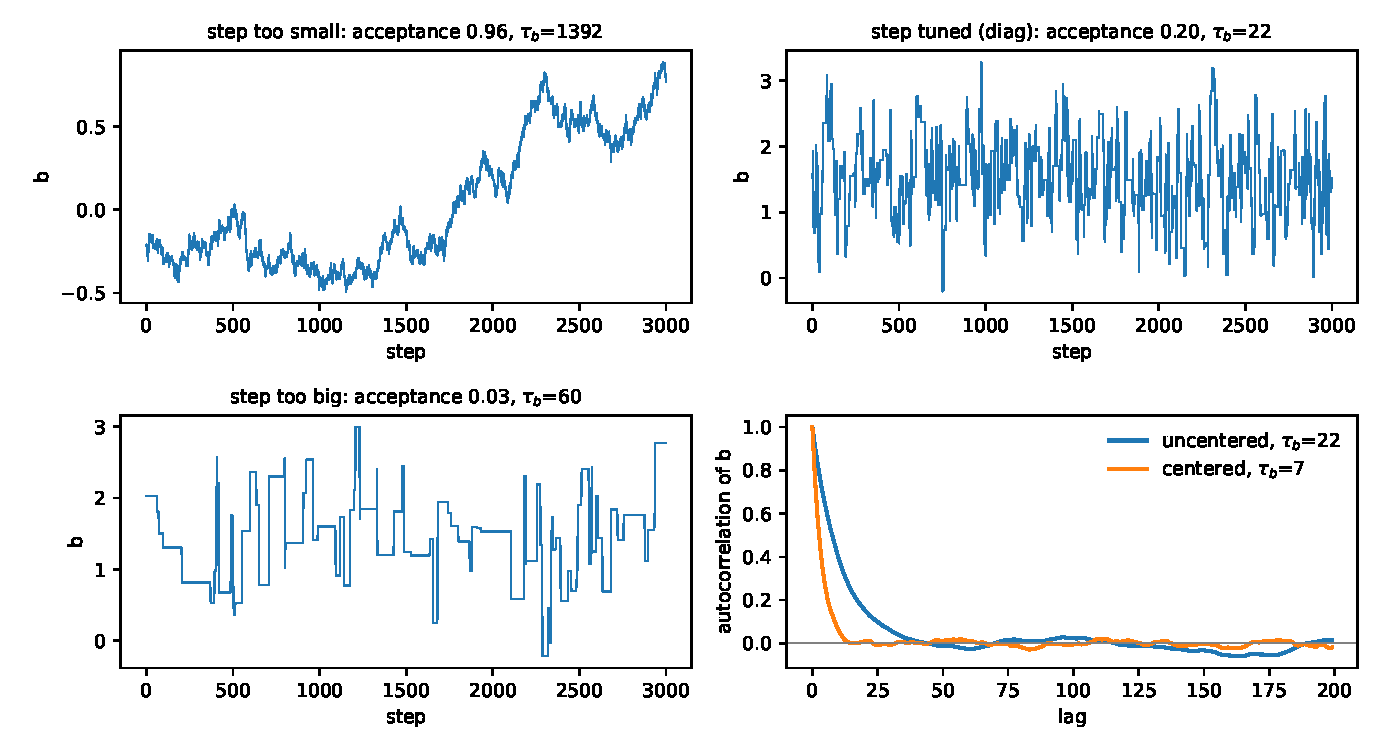
\includegraphics[width=0.49\textwidth]{figs/fig_line_mcmc.pdf}\hfill
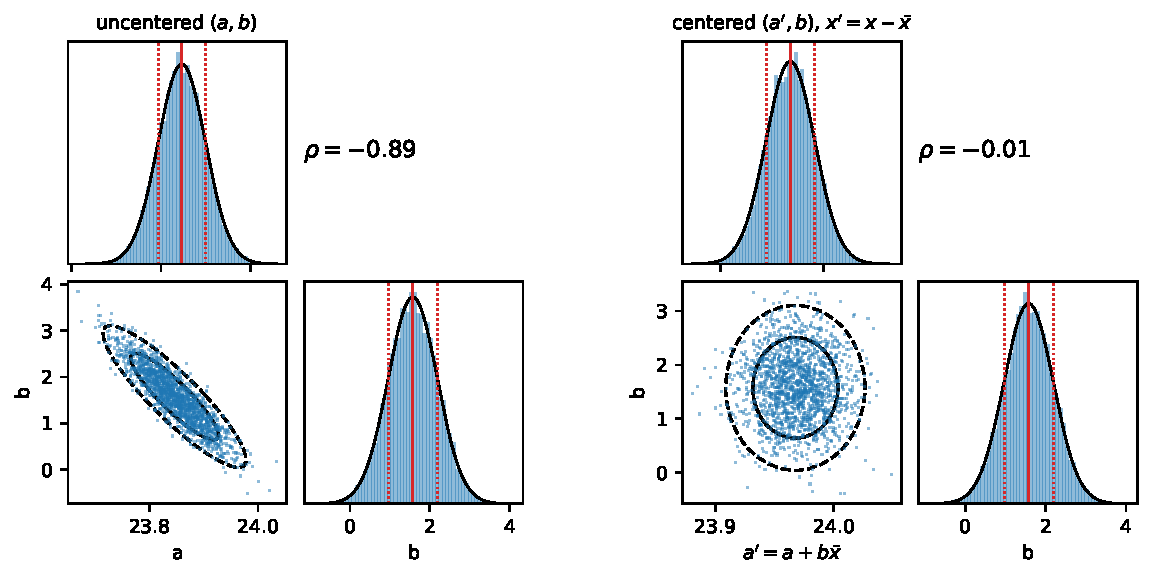
\includegraphics[width=0.42\textwidth]{figs/fig_line_corner.pdf}
\caption{\small קו ישר: עקבות השרשרת (שמאל) ו-\en{corner plot} (ימין). הדגימה משחזרת את הפתרון האנליטי, כולל $\rho_{ab}\approx-0.9$.}
\end{figure}

\subsection*{חלק ב' --- סופרנובות ואנרגיה אפלה}

\subsection{נר תקני}
סופרנובה \en{Ia}: ננס לבן שמתקרב לגבול צ'נדרסקאר ומתפוצץ. לאחר תיקוני מתיחה (\en{stretch}, $x_1$) וצבע ($c$) הבהירות בשיא אחידה ל-$\sim0.1$ מג'. מודול המרחק:
\begin{equation}
m_B=M_B+\mu(z),\qquad \mu=5\log_{10}\frac{D_L}{10\,\mathrm{pc}}=5\log_{10}\frac{D_L}{\Mpc}+25 .
\end{equation}
כותבים $D_L=(c/H_0)\,\hat D_L(z;\Omega_m,w)$. אז
\begin{equation}
m_B=\underbrace{M_B+5\log_{10}\!\Big(\frac{c/H_0}{\Mpc}\Big)+25}_{\mathcal M}+5\log_{10}\hat D_L(z;\boldsymbol\theta) .
\end{equation}
\begin{warnbox}
\textbf{$H_0$ ו-$M_B$ מופיעים רק בצירוף $\mathcal M$.} סופרנובות לבדן מודדות את \emph{צורת} $D_L(z)$, כלומר $\Omega_m,w$, ולא את $H_0$. כדי לקבל $H_0$ צריך לכייל את $M_B$ בעזרת צפייניים --- ושם נולד מתח האבל (הרצאה 5).
\end{warnbox}

\textbf{1998.} ב-$z=0.5$ ההפרש ב-$\mu$ בין \en{EdS} ל-$\LCDM$ הוא $\sim0.4$ מג': הסופרנובות הרחוקות \emph{חלשות} מהצפוי (תרגיל 2.3). זו התגלית (\en{Riess et al.\ 1998; Perlmutter et al.\ 1999}).

\subsection{מרג'ינליזציה אנליטית על $\mathcal M$}
$\mathcal M$ נכנס לינארית. עם $\mathbf r_0=\mathbf m_B-\boldsymbol\mu_{\rm th}$:
\begin{equation}
\chi^2(\mathcal M)=A-2\mathcal MB+\mathcal M^2S,\quad A=\mathbf r_0^{\!\top}\mathsf C^{-1}\mathbf r_0,\ \ B=\mathbf 1^{\!\top}\mathsf C^{-1}\mathbf r_0,\ \ S=\mathbf 1^{\!\top}\mathsf C^{-1}\mathbf 1 .
\end{equation}
אינטגרל גאוסי על $\mathcal M$ (מוקדמת אחידה) נותן
\begin{equation}
\boxed{\;\chi^2_{\rm marg}=A-\frac{B^2}{S}\;}\qquad(+\ \text{קבוע}),\qquad \hat{\mathcal M}=B/S .
\end{equation}
פרמטר אחד פחות לדגום, ושרשרת מהירה פי 2 (בדיקה בסעיף 19 במחברת).

\subsection{התוצאות}
\begin{center}\small
\begin{tabular}{@{}p{2.3cm}p{2.3cm}p{11.2cm}@{}}
\toprule
מודל & פרמטרים & תוצאה (\en{Pantheon+}, 1590 \en{SNe}, $z>0.01$) \\ \midrule
$\LCDM$ שטוח & $\Omega_m$ & $\Omega_m=0.332\pm0.018$, \ $\chi^2=1403$ ל-1589 ד"ח \\
$w$\en{CDM} שטוח & $\Omega_m,w$ & $\Omega_m=0.29^{+0.07}_{-0.08}$, $w=-0.90^{+0.14}_{-0.16}$, $\rho=-0.94$; $\Delta\mathrm{BIC}=+6.9$ לטובת $\Lambda$ \\
$\Lambda$ עקום & $\Omega_m,\Omega_\Lambda$ & $q_0=-0.47\pm0.06$ \ ($P(q_0<0)\approx1$), \ $\Omega_k=0.09\pm0.13$ \\ \bottomrule
\end{tabular}
\end{center}

\begin{figure}[htbp]\centering
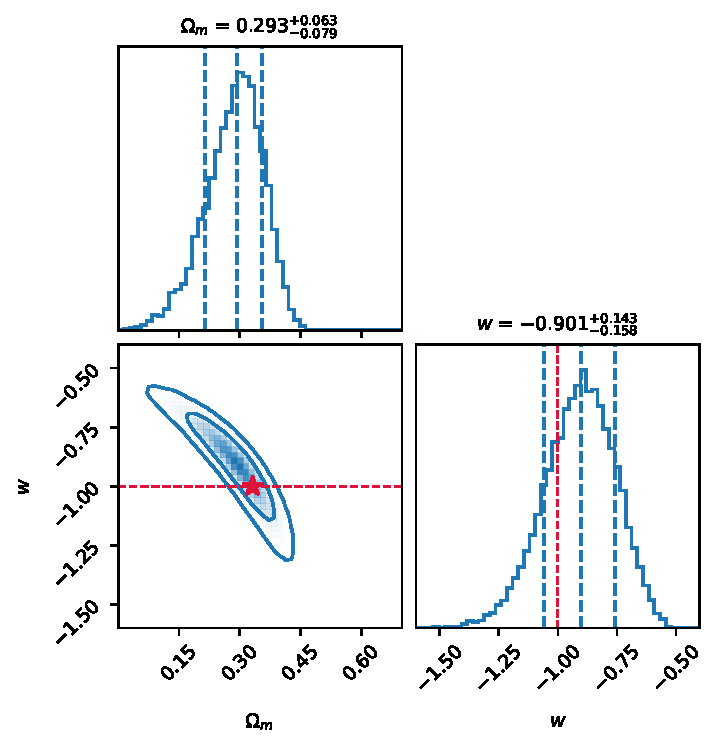
\includegraphics[width=0.38\textwidth]{figs/fig_pp_wcdm.pdf}\hfill
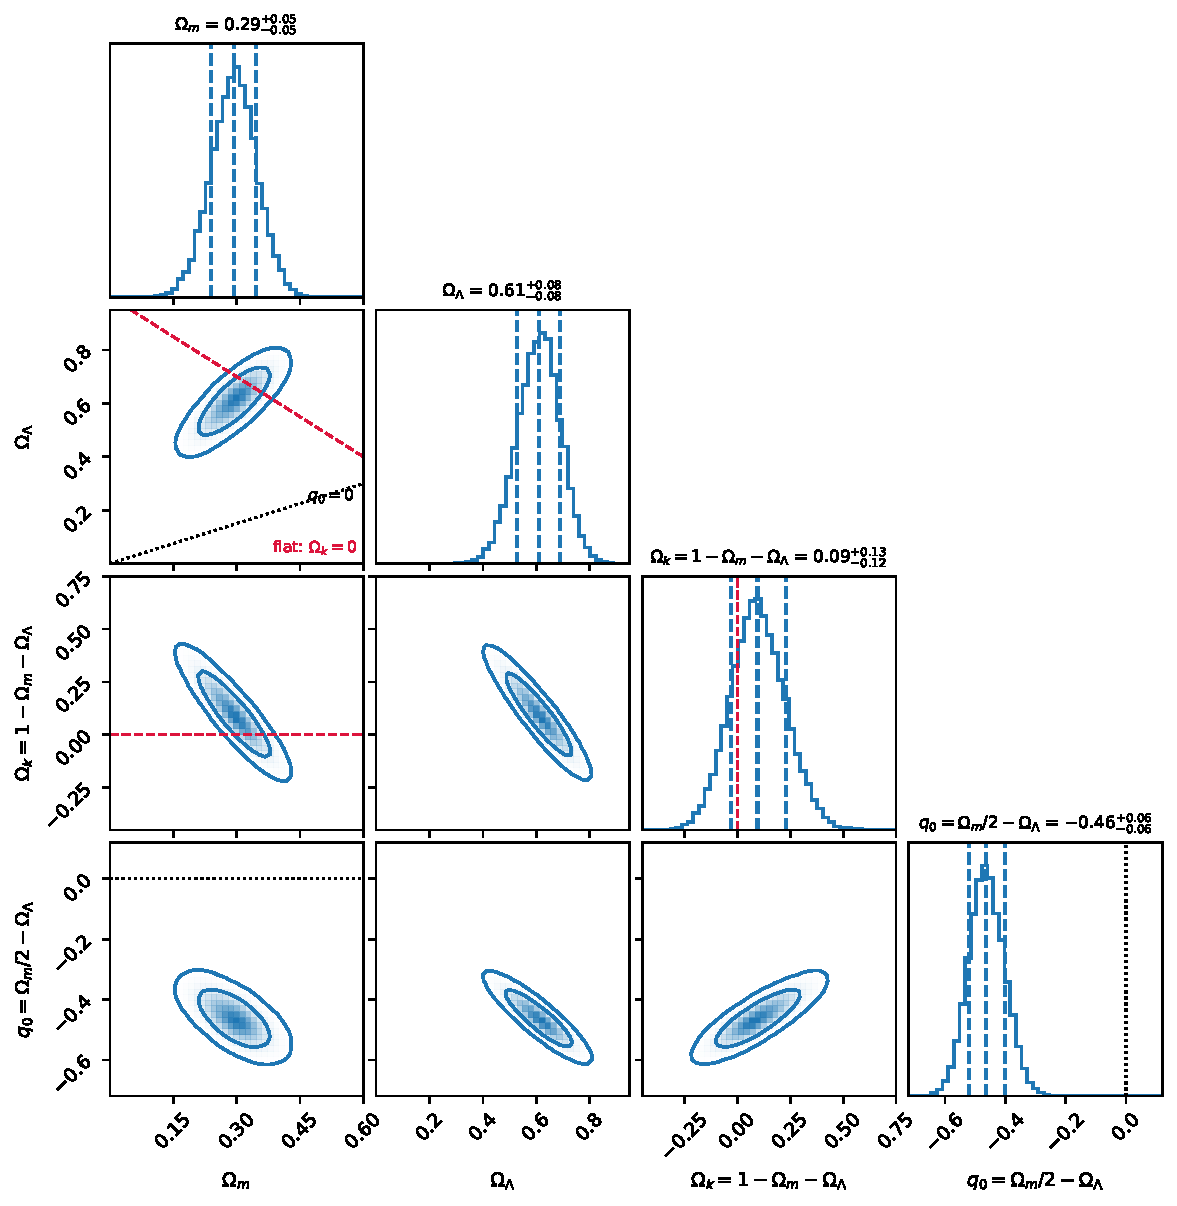
\includegraphics[width=0.40\textwidth]{figs/fig_pp_curved.pdf}
\caption{\small \en{Pantheon+}: ניוון $\Omega_m$--$w$ (שמאל) ומישור $\Omega_m$--$\Omega_\Lambda$ עם הפרמטרים הנגזרים $\Omega_k$, $q_0$ (ימין). התאוצה ($q_0<0$) איתנה; הערך של $\Omega_k$ לא.}
\end{figure}

\textbf{קריאה.} ($\Omega_m,w$): הנתונים מודדים צירוף אחד --- הגדלת $\Omega_m$ מפוצה בהקטנת $w$. ($\Omega_m,\Omega_\Lambda$): בטווח $z$ הנמוך מודדים בעיקר $q_0=\Omega_m/2-\Omega_\Lambda$. את הניוון שוברים עם \en{CMB} ו-\en{BAO} (הרצאה 5).

\subsection{סיור במחברת \en{MCMC\_Pantheon\_he}}
המחברת בונה את המכונה פעם אחת, על קו ישר שבו אפשר לבדוק הכול אנליטית, ואז מחליפה רק את המודל.
\begin{center}\small
\begin{tabular}{@{}p{2.2cm}p{5.3cm}p{7.2cm}@{}}
\toprule
סעיפים & מה קורה & מה להראות בכיתה \\ \midrule
1--2 & נתונים סינתטיים, פתרון אנליטי (מטריצת פישר $F=A^{\!\top}A/\sigma^2$) & $\rho_{ab}=-0.90$: הנתונים רחוקים מהראשית \\
3 & \texttt{log\_prior}, \texttt{log\_likelihood}, \texttt{log\_probability} & החזרת $-\infty$ $=$ "אסור"; למה לוגריתם \\
4--5 & איתחול 32 הולכים בכדור קטן סביב המקסימום; \texttt{run\_mcmc} & צורת השרשרת \texttt{(nsteps, nwalkers, ndim)} \\
6 & עקבות, $\tau\approx32$, \en{burn-in} $=5\tau$, $\hat R$ מ-4 ריצות & $N_{\rm eff}\approx5900$; $\hat R-1<10^{-3}$ \\
7--8 & \en{corner}; 60 קווים מהמאוחרת & הדגימה $=$ האנליטי; ה"צוואר" ב-$\bar x$ \\
9--10 & מרכוז $x'=x-\bar x$; קיבוע מול מרג'ינליזציה & קיבוע מקטין $\sigma_b$ פי $2.34=1/\sqrt{1-\rho^2}$ \\
11 & קו מול פרבולה: \en{AIC/BIC} & $\Delta\mathrm{BIC}=+3.1$: הקו מספיק \\ \midrule
12--13 & \en{Pantheon+}: \texttt{zHD}, \texttt{zHEL}, \texttt{m\_b\_corr}, מטריצת שונות מלאה & הופכים את $\mathsf C$ \emph{פעם אחת} לפני הריצה \\
14 & $\mu(z)$ על רשת $z$ צפופה + \texttt{np.interp} & מהיר פי מאות מ-\texttt{quad} לכל סופרנובה \\
15 & $\chi^2_{\rm marg}=A-B^2/S$ & \en{EdS}: $\chi^2=2101$; $\LCDM$: $1403$ \\
16 & $\LCDM$: רשת מול \en{emcee} & $\Omega_m=0.332\pm0.018$ בשתי הדרכים \\
17 & $w$\en{CDM} & בננה, $\rho=-0.94$, $P(w<-1)=0.27$ \\
18 & עקום; פרמטרים נגזרים שורה-שורה & $q_0<0$ בלי "התפשטות שגיאות" \\
19 & דגימה מפורשת של $\mathcal M$ & אותה תוצאה; $\tau$ גדל פי 2 \\ \bottomrule
\end{tabular}
\end{center}

הלב של כל הניתוח --- שלוש פונקציות קצרות:
\begin{otherlanguage}{english}
\begin{lstlisting}
def chi2_marg(mu):                      # analytic marginalisation over M
    r0 = mb - mu
    A = r0 @ (Cinv @ r0); B = s_vec @ r0   # s_vec = Cinv@1, S_sum = 1^T Cinv 1
    return A - B*B/S_sum

def log_prob_wcdm(theta):
    Om, w = theta
    if not (0 < Om < 1 and -3 < w < 0): return -np.inf    # flat prior
    mu = mu_model(Om, w)
    return -np.inf if mu is None else -0.5*chi2_marg(mu)

sampler = emcee.EnsembleSampler(32, 2, log_prob_wcdm)
sampler.run_mcmc(best + 1e-2*rng.normal(size=(32, 2)), 4000)
\end{lstlisting}
\end{otherlanguage}

% ---------------------------------------------------------------------
\subsection*{תרגילים}
\begin{exercise}{קו ישר אנליטית}
$N$ נקודות $y_i=a+bx_i$ עם שגיאה $\sigma$. (א) כתבו את $\chi^2$ והראו שמטריצת פישר היא $F=\frac{N}{\sigma^2}\begin{pmatrix}1&\bar x\\ \bar x&\overline{x^2}\end{pmatrix}$. (ב) הראו ש-$\rho_{ab}=-\bar x/\sqrt{\overline{x^2}}$. (ג) הראו שהשגיאה השולית על $b$ גדולה מהשגיאה המותנית (כש-$a$ מקובע) בפקטור $1/\sqrt{1-\rho^2}$. מה זה אומר על תכנון סקר סופרנובות?
\end{exercise}
\begin{solbox}
\textbf{פתרון.}\ (א) $F_{ij}=\tfrac12\partial_i\partial_j\chi^2$: $F_{aa}=N/\sigma^2$, $F_{ab}=N\bar x/\sigma^2$, $F_{bb}=N\overline{x^2}/\sigma^2$.\\
(ב) ל-$2\times2$, $C=F^{-1}$ ו-$\rho=C_{ab}/\sqrt{C_{aa}C_{bb}}=-F_{ab}/\sqrt{F_{aa}F_{bb}}=-\bar x/\sqrt{\overline{x^2}}$.\\
(ג) $\sigma_b^2(\text{שולי})=C_{bb}=F_{aa}/\det F$, $\sigma_b^2(\text{מותנה})=1/F_{bb}$. היחס: $F_{aa}F_{bb}/\det F=1/(1-\rho^2)$. בסקר: זרוע ארוכה בהסחה, ומדגם עוגן ב-$z$ נמוך, כדי לשבור את הקורלציה עם ההיסט $\mathcal M$. (במחברת: $\rho=-0.90$, יחס $2.34$.)
\end{solbox}

\begin{exercise}{מרג'ינליזציה על ההיסט}
(א) בצעו את האינטגרל $\int e^{-\chi^2(\mathcal M)/2}d\mathcal M$ עם $\chi^2=A-2\mathcal MB+\mathcal M^2S$ והראו ש-$\chi^2_{\rm marg}=A-B^2/S+\ln(S/2\pi)$. (ב) הראו שזה שווה (עד קבוע) ל-$\chi^2$ המינימלי על $\mathcal M$ (\en{profile}). למה זה נכון כאן ולא באופן כללי? (ג) כש-$\mathsf C$ אלכסונית, מה $\hat{\mathcal M}$?
\end{exercise}
\begin{solbox}
\textbf{פתרון.}\ (א) השלמה לריבוע: $\chi^2=S(\mathcal M-B/S)^2+A-B^2/S$. האינטגרל הגאוסי נותן $\sqrt{2\pi/S}\,e^{-(A-B^2/S)/2}$, ולכן $-2\ln=A-B^2/S+\ln(S/2\pi)$.\\
(ב) המינימום על $\mathcal M$ ב-$\hat{\mathcal M}=B/S$ נותן בדיוק $A-B^2/S$. השוויון נובע מכך שהנראות גאוסית בפרמטר לינארי, $S$ לא תלוי ב-$\boldsymbol\theta$ (מטריצת שונות קבועה) והמוקדמת אחידה. בפרמטר לא-לינארי, או כש-$\mathsf C$ תלויה בפרמטרים, מרג'ינליזציה ופרופיל שונים (הבדל "נפח").\\
(ג) $\hat{\mathcal M}=\sum_i(r_{0,i}/\sigma_i^2)\big/\sum_i\sigma_i^{-2}$: ממוצע משוקלל של השאריות.
\end{solbox}

\begin{exercise}{כמה חלשות הסופרנובות?}
(א) חשבו $\Delta\mu=\mu_{\LCDM}-\mu_{\rm EdS}$ ב-$z=0.5$ עבור $\Omega_m=0.3$ (אינטגרל נומרי פשוט, או סימפסון בשלוש נקודות). (ב) עם פיזור $0.15$ מג' לסופרנובה, כמה סופרנובות ב-$z\approx0.5$ נחוצות כדי להבחין בין המודלים ב-$5\sigma$? (ג) למה מספיק לדעת את $\Delta\mu$ ולא את $H_0$?
\end{exercise}
\begin{solbox}
\textbf{פתרון.}\ (א) $\int_0^{0.5}dz/E=0.441$ ($\LCDM$) מול $2(1-1.5^{-1/2})=0.367$ (\en{EdS}). $\Delta\mu=5\log_{10}(0.441/0.367)=+0.40$ מג': ב-$\LCDM$ הסופרנובות חלשות יותר.\\
(ב) $\mathcal M$ לא ידוע, ולכן משווים ממוצע ב-$z\approx0.5$ לממוצע ב-$z$ נמוך: $\sigma_{\Delta}=0.15\sqrt{2/N}<0.40/5$ נותן $N\gtrsim7$ בכל סל. בפועל השגיאות השיטתיות (כיול, אבק, אבולוציה) $\sim0.02$--$0.03$ מג' הן הגבול, לא $N$.\\
(ג) $H_0$ מוסיף קבוע ל-$\mu$ בכל $z$. ההבחנה היא בצורת $\mu(z)$, יחסית ל-$z$ נמוך.
\end{solbox}
